\documentclass[letterpaper, 12pt]{article}
\usepackage[margin=1in]{geometry}
\usepackage{amsmath}
\usepackage{amssymb}
\usepackage{tikz}
\usepackage{pgfplots}
\usepackage{fancyhdr}

\pagestyle{fancy}
\fancyhf{}

\rhead{
    Shengdong Li
    Table 7
    Calc 1
}
\rfoot{Page \thepage}

\usepackage{indentfirst}
\setlength{\parindent}{2em}
\setlength{\parskip}{1em}

\begin{document}
\title{To Conclude}
\author{by Shengdong Li}
\date{5 April 2020}
\maketitle

\section{Abstract}
This discussion has taught me a lot about the usefulness of trig identies and proofs, and has helped refine my $u$-substitution technique. I also learned a lot about latex editors and the latex language.
\section{Initial Post}
To integrate $\int\sin x\cos^2 x\:dx$, I first $u$-subbed using $u = \sin x$, then $u = \cos x$, leaving me with
$\frac{1}{2}\sin^2x+c\:\:\:\text{and}\:\:-\frac{1}{2}\cos^2x+c$. \par
To try and prove that the two expressions were equal, I graphed them without the $c$ value, which looked like this: \par
\begin{center}
    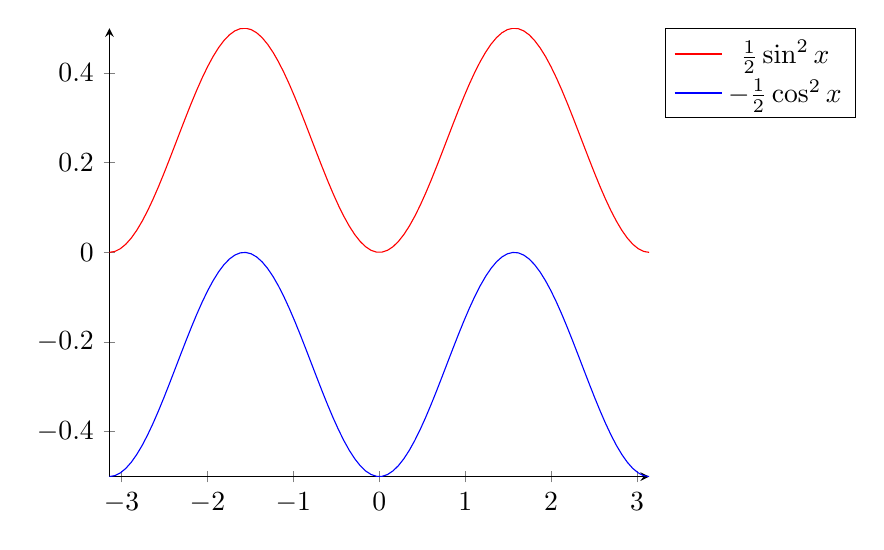
\begin{tikzpicture}
        \begin{axis}[
                axis lines = left,
                domain=-3.14:3.14,
                legend pos=outer north east
            ]
            \addplot [mark=none, color=red, samples=100]{(1/2)*(sin(deg(x)))^2};
            \addplot [mark=none, color=blue, samples=100]{-(1/2)*(cos(deg(x)))^2};
            \legend{$\frac{1}{2}\sin^2x$, $-\frac{1}{2}\cos^2x$}
        \end{axis}
    \end{tikzpicture}
\end{center}
Then I was able to conclude that the two expressions were equal, since evidently they were the same equations ignoring the horizontal shift differences, which could be anything since the $c$ values were not known.
\section{Comments on My Post}
Through the comments of Max Shi and Ali Fahkry, I realized that there were two more ways that the expressions could be proved to equal.\par
One way was using the trig identity $\sin^2x+\cos^2x=1$, and plugging in  $\sin^2x=1-\cos^2x$ or $\cos^2x=1-\sin^2x$ into $\frac{1}{2}\sin^2x+c$ or
$-\frac{1}{2}\cos^2x+c$ respectively, which resulted in the other equation exactly. This method is probably better than the graphing method, in which only a portion of the graph could ever be shown. \par
Another way to explain the equality of the two expressions was to just set them equal to one another, and through the use of the trig identity $\sin^2x+\cos^2x=1$ again, everything cancelled and only the difference of the two $c$ values from either equation were left, which was $\frac{1}{2}$. This proved equality because the $c$ values are not known, and as shown earlier, the cosine graph shifted $\frac{1}{2}$ up was just the sine graph.
\section{Checking Work}
Finally, evaluating $\int\sin x\cos^2x\:dx$ was pretty fun. Using $u=\sin x$, the integration was straghtforward. However, using $u=\cos x$ required the manipulation of the original equation using the trig identity $\sin^2x+\cos^2x=1$, in order to $u$ sub. Then, a further $v$ sub was needed to allow for integration. \par
Integrating this expression reminded me to always be on the lookout for using trig identities when integrating sinusoids, and gave me more hints for when a double variable substitution was needed.
\section{Latex}
Using a latex editor has changed my life. It has made me \textit{want} to show my work more, and spend more time on calc discussions. I feel like I can put out better-looking comments in future discussions, with improved efficiency.
\section{In Conclusion Conclusion}
This discussion has reminded me of how important the $\sin^2x+\cos^2x=1$ identity is in evaluating integrals, while pushing me to learn latex, an important skill that I feel will be utilized later down the line. \par
Until the next discussion,
Shengdong Li
\end{document}